\documentclass[tikz]{standalone}

\usepackage[british]{babel}
\usepackage[utf8]{inputenc}
\usepackage{graphicx}
\usepackage{amsmath}
\usepackage{amssymb}
\usepackage{amsfonts}
\usepackage{bm}
\usepackage{color}
\usepackage[unicode]{hyperref}
\usepackage{multirow}
\usepackage{multicol}
\usepackage{tikz}
\usepackage{hyperref} % this is for url links
\usepackage{textcomp}
\usepackage{pgfplots}

\usetikzlibrary{arrows,shapes, calc}

\pgfplotsset{colormap={parula}{
        rgb255=(53,42,135)
        rgb255=(15,92,221)
        rgb255=(18,125,216)
        rgb255=(7,156,207)
        rgb255=(21,177,180)
        rgb255=(89,189,140)
        rgb255=(165,190,107)
        rgb255=(225,185,82)
        rgb255=(252,206,46)
        rgb255=(249,251,14)}}


\begin{document}

\def\figscale{2}
\setlength\textwidth{17.2cm}

\begin{tikzpicture}[scale=2]
    \def\figw{0.15\textwidth}
    \node [below left, inner sep=0] (img1) at (0,0) {\includegraphics[width=\figw]{figs/wulff_sketch/sketch_Wulff_4fold_soa0-04.pdf}};
    \node [below right, inner sep=0] (img2) at (img1.north east) {\includegraphics[width=\figw]{figs/wulff_sketch/sketch_Wulff_4fold_soa0-40.pdf}};
    \node [below right, inner sep=0] (img3) at (img2.north east) {\includegraphics[width=\figw]{figs/wulff_sketch/sketch_Wulff_4fold_soa0-70.pdf}};
    
    \draw[above, inner sep=0] (img1.north west) node {(a)};
    \draw[above, inner sep=0] (img2.north west) node {(b)};
    \draw[above, inner sep=0] (img3.north west) node {(c)};

    \draw[above, inner sep=0] (img1.north) node {$\delta=0.04$};
    \draw[above, inner sep=0] (img2.north) node {$\delta=0.4$};
    \draw[above, inner sep=0] (img3.north) node {$\delta=0.7$};
    
\end{tikzpicture}

\begin{tikzpicture}
    \def\figw{0.2\textwidth}
    \node [below left, inner sep=0] (img1) at (0,0) {\includegraphics[width=\figw]{figs/wulf_cross_orders/Wulff_cross_order_0_6fold_soa0-70.pdf}};
    \node [below right, inner sep=0] (img2) at (img1.north east) {\includegraphics[width=\figw]{figs/wulf_cross_orders/Wulff_cross_order_1_6fold_soa0-70.pdf}};
    \node [below left, inner sep=0] (img3) at (img1.south east) {\includegraphics[width=\figw]{figs/wulf_cross_orders/Wulff_cross_order_2_6fold_soa0-70.pdf}};
    \node [below right, inner sep=0] (img4) at (img3.north east) {\includegraphics[width=\figw]{figs/wulf_cross_orders/Wulff_cross_order_3_6fold_soa0-70.pdf}};
    
    \draw[above, inner sep=0] (img1.north west) node {(a)};
    \draw[above, inner sep=0] (img2.north west) node {(b)};
    \draw[above, inner sep=0] (img3.north west) node {(c)};
    \draw[above, inner sep=0] (img4.north west) node {(d)};

    \draw[above, inner sep=0] (img2.north) node {cross order 1};
    \draw[above, inner sep=0] (img3.north) node {cross order 2};
    \draw[above, inner sep=0] (img4.north) node {cross order 3};
    
\end{tikzpicture}

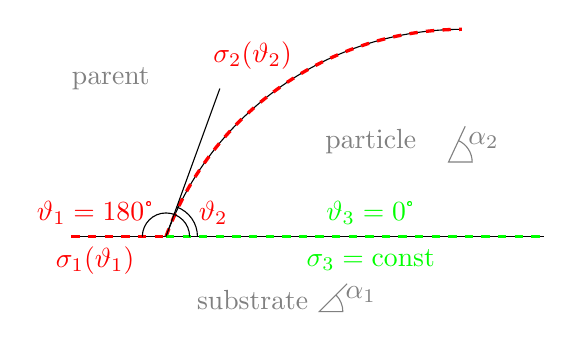
\begin{tikzpicture}
    \draw (-3,0) -- (3,0);
    \draw (-1.8,0) arc (160:90:4);
    \draw[dashed,very thick,red] (-1.8,0) arc (160:90:4);
    \draw[dashed,very thick,red] (-3,0) -- (-1.8,0);
    \draw[dashed,very thick,green] (-1.8,0) -- (3,0);
    
    \draw[gray] (-0.7,-0.8) node {substrate};
    \draw[gray] (0.5,-0.6) -- ++(-135:0.5) -- ++(0.3,0) arc (0:45:0.3) node[right] {$\alpha_1$};
    \draw[gray] (0.8,1.2) node {particle};
    \draw[gray] (2,1.4) -- ++(-115:0.5) -- ++(0.3,0) arc (0:65:0.3) node[right] {$\alpha_2$};
    \draw[gray] (-2.5,2) node {parent};
    
    \draw (-1.8,0) -- +(70:2);
    \draw (-1.8+0.4,0) arc (0:70:0.4);
    \draw[red] (-1.2,0.3) node {$\vartheta_2$};
    \draw[red] (-0.7,2.3) node {$\sigma_2(\vartheta_2)$};
    \draw[red] (-2.7,0.3) node {$\vartheta_1 = 180$\textdegree};
    \draw[red] (-2.7,-0.3) node {$\sigma_1(\vartheta_1)$};
    \draw (-1.8+0.3,0) arc (0:180:0.3);
    
    \draw[green] (0.8,0.3) node {$\vartheta_3=0$\textdegree};
    \draw[green] (0.8,-0.3) node {$\sigma_3=\mathrm{const}$};
\end{tikzpicture}



\begin{tikzpicture}
    \node [above right, inner sep=0] (img1) at (0,0) {\includegraphics[page=2,width=0.4\textwidth]{sketches.pdf}};
    % \node [below right, inner sep=0] (img2) at (0,0) {\includegraphics[page=3,width=0.4\textwidth]{sketches.pdf}};
    
    % \draw[above, inner sep=0] (img1.north west) node {(a)};
    % \draw[above, inner sep=0] (img2.north west) node {(b)};
    
\end{tikzpicture}


\begin{tikzpicture}
    
	\def\figw{0.23\textwidth}

    \node [below right, inner sep=0] (img0) at (0,0) {\includegraphics[width=\figw]{figs/SF/S_4fold_isotropic.pdf}};
    \node [below right, inner sep=0] (img1) at (img0.north east) {\includegraphics[width=\figw]{figs/SF/S_4fold_soa0-10.pdf}};
    % \node [below right, inner sep=0] (img2) at (img1.north east) {\includegraphics[width=\figw]{figs/SF/S_4fold_soa0-40.pdf}};
    \node [below, inner sep=0.2cm] (img2) at (img0.south) {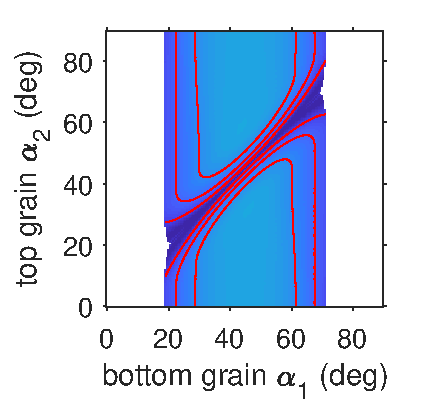
\includegraphics[width=\figw]{figs/SF/S_4fold_soa0-50.pdf}};
    \node [below, inner sep=0.2cm] (img3) at (img1.south) {\includegraphics[width=\figw]{figs/SF/S_4fold_soa0-70.pdf}};
    
    % \node [below right, inner sep=0] (img2) at (img1.north east) {\includegraphics[page=3,width=\figw]{sketches.pdf}};

    \draw[above, inner sep=0] (img0.north west) node {(a)};
    \draw[above, inner sep=0] (img1.north west) node {(b)};
    \draw[below, inner sep=0] (img0.south west) node {(c)};
    \draw[below, inner sep=0] (img1.south west) node {(d)};

    \draw[above, inner sep=0] (img0.north) node {$\delta=0$};
    \draw[above, inner sep=0] (img1.north) node {$\delta=0.1$};
    \draw[below, inner sep=0] (img0.south) node {$\delta=0.5$};
    \draw[below, inner sep=0] (img1.south) node {$\delta=0.7$};
    
    % https://tex.stackexchange.com/questions/247940/parula-colormap-in-pgfplots
    \node [left, inner sep=0.2cm] (clrbar) at (img0.south west) {\pgfplotscolorbardrawstandalone[
    	colormap access=piecewise const,
    	colorbar sampled,
    	colorbar style={ytick={0,0.25,...,2.5},samples=11,width=0.2cm,height=3cm},
    	point meta min=0,
    	point meta max=2.5,
    	y tick label style={font=\footnotesize},
    	% axis line style={draw=none},
    	% tick style={draw=none},
    	% xticklabels=\empty,
    	% yticklabels=\empty,
    	]
    	% \pgfplotsset{y tick label style={font=\tiny}}
    	% \end{axis}
    	};
    
\end{tikzpicture}


\begin{tikzpicture}
    % \node [above, inner sep=0.5cm] (img1) at (0,0) {\includegraphics[page=4,width=0.1\textwidth]{sketches.pdf}};
    \node [below, inner sep=0] (img2) at (0,0) {\includegraphics[width=0.45\textwidth]{sketches/MC_scheme_vertical.pdf}};
    
    % \draw[below left, inner sep=0.5cm] (img1.north west) node {(a)};
    % \draw[above, inner sep=0] (img2.north west) node {(b)};
    
\end{tikzpicture}


\tikzstyle{redstop} = [circle, draw, white,minimum size=1.5mm,line width = 1mm,fill=red, inner sep=0]
\begin{tikzpicture}[font = \footnotesize]
    \def\scaleconst{0.6}
    \node [above right, inner sep=0] (img1) at (0,0) {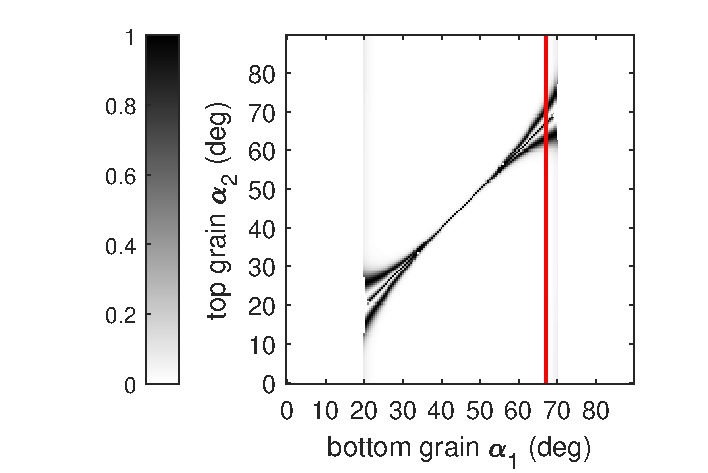
\includegraphics[scale=\scaleconst,trim={1.5cm 0 0 0},clip]{figs/MC/nucleation_sampling_Pmap.pdf}};
    \node [above right, inner sep=0] (img2) at (img1.south east) {\includegraphics[scale=\scaleconst]{figs/MC/nucleation_sampling_cdf.pdf}};

    \draw[right, inner sep=0cm] (img1.north west) node {\normalsize (a)};
    \draw[right, inner sep=0] (img2.north west) node {\normalsize (b)};

    \begin{scope}[
            x={($0.025*(img2.south east)$)},
            y={($0.025*(img1.north west)$)}]
        % % Grid
        % \draw[green,step=1] (img1.south west) grid (img2.north east);
        % % axis labels
        % \foreach \x in {0,1,...,40} { \node [below] at (\x,0) {\tiny\x}; }
        % \foreach \y in {0,1,...,40} { \node [left] at (0,\y) {\tiny\y};}


        \draw[red,|-stealth] (13.77,-3)  node[above] {initial $\alpha_1$} |- (23.7,-7) node[redstop] {} -- (29.7,-7) node[redstop] {} -- (35.9,-7);
        \draw (36.3,-7) node[redstop] {};
        % \node (cdf_pt) at (9,5) {};
        \fill[blue,circle]  (36.3,30.2) circle (1.5pt);
        % \node[draw,blue,circle,fill=blue] (cdf_pt) at (2*18,8) {};
        \draw[blue,-stealth] (36.3,30.2) -> (33.6,30.2) ;
        \draw[blue,-stealth] (19,30.2) -| (14.1,8);
        % \draw[red,-stealth,dashed] (17.5,-8) node[below] {\footnotesize initial orientation} -> (17.5,3);
        % \draw[blue,-stealth,dashed] (18,2) .. controls  +(-45:4) and +(180:4)  .. (28,-3);
        \draw[blue,-stealth] (23.7,-5) -> (23.7,-1) node[midway,right] {$\xi_3$} ;
        \draw[blue] (29.7,-4.3) node[above,inner sep=0] {$\xi_3=0.5$} ;
        \draw[blue,-stealth] (36.3,-5) -> (36.3,-1) node[midway,right] {$\xi_4$} -> (36.3,29) ;
        
        
    \end{scope}
\end{tikzpicture}

\begin{tikzpicture}
\def\figh{3cm};
    \node [below right, inner sep=0] (img1) at (0,0) {\includegraphics[height=\figh,trim={1.5cm 0 0.2cm  0},clip]{figs/MC/mean_events_ICA_IN.pdf}};
    \node [below right, inner sep=0] (img2) at (img1.north east) {\includegraphics[height=\figh, trim={4cm 0 0.2cm  0},clip]{figs/MC/mean_events_ICA_AN.pdf}};
    \node [below, inner sep=0] (img4) at ($(img2.south)+(0,-0.2cm)$) {\includegraphics[height=\figh,trim={4cm 0 0.2cm  0},clip]{figs/MC/mean_events_ICH_AN.pdf}};
    \node [left, inner sep=0] (img3) at (img4.west) {\includegraphics[height=\figh, trim={4cm 0 0.2cm  0},clip]{figs/MC/mean_events_ICL_AN.pdf}};

    \draw[ right, inner sep=1.5cm] (img1.north west) node {(a) IC\_A IN};
    \draw[ right, inner sep=0] (img2.north west) node {(b) IC\_A AN};
    \draw[ right , inner sep=0] (img3.north west) node {(c) IC\_L AN};
    \draw[ right, inner sep=0] (img4.north west) node {(d) IC\_H AN};

%    \def\shiftRlabel{0.5cm};
%    \draw[ left, inner sep=\shiftRlabel] (img1.north east) node {IC\_A IN};
%    \draw[ left, inner sep=\shiftRlabel] (img2.north east) node {IC\_A AN};
%    \draw[ left , inner sep=\shiftRlabel] (img3.north east) node {IC\_L AN};
%    \draw[ left, inner sep=\shiftRlabel] (img4.north east) node {IC\_H AN};
    
\end{tikzpicture}

\begin{tikzpicture}
\def\figheight{2.5cm};
\def\vspacing{0.4cm};

    \node [below right, inner sep=0] (img11) at (0,0) {\includegraphics[height=\figheight, trim={0.2cm 0 0.5cm  0},clip]{figs/MC/fig11_deposit_ NN_soa5e-01_exphom10_ind103_repnum2_nucl-sites-on.pdf}};
    \node [below right, inner sep=0] (img12) at (img11.north east) {\includegraphics[height=\figheight, trim={1cm 0 2cm  0},clip]{figs/MC/fig11_ori_distrib_thru_thick_NN_soa5e-01_exphom10_ind103.pdf}};

    \node [below right, inner sep=0] (img21) at ($(img11.south west)+(0,-\vspacing)$) {\includegraphics[trim={0.2cm 0 0.5cm 0},clip,height=\figheight]{figs/MC/fig12_deposit_ IN_soa5e-01_exphom30_ind153_repnum2_nucl-sites-on.pdf}};
    \node [below right, inner sep=0] (img22) at (img21.north east) {\includegraphics[height=\figheight, trim={1cm 0 2cm  0},clip]{figs/MC/fig12_ori_distrib_thru_thick_IN_soa5e-01_exphom30_ind153.pdf}};

    \node [below right, inner sep=0] (img31) at ($(img21.south west)+(0,-\vspacing)$) {\includegraphics[trim={0.2cm 0 0.5cm 0},clip,height=\figheight]{figs/MC/fig13_deposit_ AN_soa5e-01_exphom30_ind154_repnum2_nucl-sites-on.pdf}};
    \node [below right, inner sep=0] (img32) at (img31.north east) {\includegraphics[height=\figheight, trim={1cm 0 2cm  0},clip]{figs/MC/fig13_ori_distrib_thru_thick_AN_soa5e-01_exphom30_ind154.pdf}};
    
    \draw[above right, inner sep=0] (img11.north west) node {(a) NN, IC\_A, $\beta=30$};
    \draw[above right, inner sep=0] (img12.north west) node {(b)};
    \draw[above right, inner sep=0] (img21.north west) node {(c) IN, IC\_A, $\beta=30$};
    \draw[above right, inner sep=0] (img22.north west) node {(d)};
    \draw[above right, inner sep=0] (img31.north west) node {(e) AN, IC\_A, $\beta=30$};
    \draw[above right, inner sep=0] (img32.north west) node {(f)};
\end{tikzpicture}

\begin{tikzpicture}
\def\figheight{2.5cm};
\def\vspacing{0.4cm};

    \node [below right, inner sep=0] (img11) at (0,0) {\includegraphics[height=\figheight, trim={0.2cm 0 0.5cm  0},clip]{figs/MC/fig21_deposit_ NN_soa5e-01_exphom90_ind223_repnum2_nucl-sites-on.pdf}};
    \node [below right, inner sep=0] (img12) at (img11.north east) {\includegraphics[height=\figheight, trim={1cm 0 2cm  0},clip]{figs/MC/fig21_ori_distrib_thru_thick_NN_soa5e-01_exphom90_ind223.pdf}};

    \node [below right, inner sep=0] (img21) at ($(img11.south west)+(0,-\vspacing)$) {\includegraphics[trim={0.2cm 0 0.5cm 0},clip,height=\figheight]{figs/MC/fig22_deposit_ AN_soa5e-01_exphom90_ind225_repnum2_nucl-sites-on.pdf}};
    \node [below right, inner sep=0] (img22) at (img21.north east) {\includegraphics[height=\figheight, trim={1cm 0 2cm  0},clip]{figs/MC/fig22_ori_distrib_thru_thick_AN_soa5e-01_exphom90_ind225.pdf}};
    
    \draw[above right, inner sep=0] (img11.north west) node {(a) NN, IC\_H, $\beta=90$};
    \draw[above right, inner sep=0] (img12.north west) node {(b)};
    \draw[above right, inner sep=0] (img21.north west) node {(c) AN, IC\_H, $\beta=90$};
    \draw[above right, inner sep=0] (img22.north west) node {(d)};
\end{tikzpicture}

\begin{tikzpicture}
\def\figheight{2.5cm};
\def\vspacing{0.4cm};

    \node [below right, inner sep=0] (img11) at (0,0) {\includegraphics[height=\figheight, trim={0.2cm 0 0.5cm  0},clip]{figs/MC/fig31_deposit_ IN_soa5e-01_exphom10_ind200_repnum2_nucl-sites-off.pdf}};
    \node [below right, inner sep=0] (img12) at (img11.north east) {\includegraphics[height=\figheight, trim={1cm 0 2cm  0},clip]{figs/MC/fig31_ori_distrib_thru_thick_IN_soa5e-01_exphom10_ind200.pdf}};

    \node [below right, inner sep=0] (img21) at ($(img11.south west)+(0,-\vspacing)$) {\includegraphics[trim={0.2cm 0 0.5cm 0},clip,height=\figheight]{figs/MC/fig32_deposit_ AN_soa5e-01_exphom10_ind201_repnum2_nucl-sites-off.pdf}};
    \node [below right, inner sep=0] (img22) at (img21.north east) {\includegraphics[height=\figheight, trim={1cm 0 2cm  0},clip]{figs/MC/fig32_ori_distrib_thru_thick_AN_soa5e-01_exphom10_ind201.pdf}};
    
    \draw[above right, inner sep=0] (img11.north west) node {(a) IN, IC\_H, $\beta=10$};
    \draw[above right, inner sep=0] (img12.north west) node {(b)};
    \draw[above right, inner sep=0] (img21.north west) node {(c) AN, IC\_H, $\beta=10$};
    \draw[above right, inner sep=0] (img22.north west) node {(d)};
\end{tikzpicture}

\begin{tikzpicture}
\def\figheight{2.3cm};
\def\figw{8cm};

    % \node [below right, inner sep=0] (img1) at (0,0) {\includegraphics[height=\figheight]{figs/SF/inverted_winterbottom_3fold.pdf}};
    % \node [below right, inner sep=0] (img2) at (img1.north east) {\includegraphics[height=\figheight]{figs/wulff_sketch/twice_inverted_winterbottom_detail.pdf}};
    
    
    % \draw[above right, inner sep=0] (img1.north west) node {(a) };
    % \draw[above right, inner sep=0] ($(img1.north west)+(3,0)$) node {(b) };
    % \draw[above right, inner sep=0] ($(img1.north west)+(6,0)$)  node {(c) };
    % \draw[above right, inner sep=0] ($(img1.north west)+(9,0)$)  node {(d) };
    % \draw[above right, inner sep=0] (img2.north west) node {(e)};

    \node [below right, inner sep=0] (img1) at (0,0) {\includegraphics[width=\figw]{figs/SF/inverted_winterbottom_3fold_narrow.pdf}};
    \draw[above right, inner sep=0] (img1.north west) node {(a) };
    \draw[above right, inner sep=0] ($(img1.north west)+(0,-5.3cm)$) node {(b) };
    \draw[inner sep=0] ($(img1.north west)+(3.4,0)$)  node[circle,minimum height=0.5cm,draw] {\small 1};
    \draw[inner sep=0]  ($(img1.north west)+(3.4,-3)$) node[circle,minimum height=0.5cm,draw] {\small 2} ;
    \draw[inner sep=0] ($(img1.north west)+(4.4,-3)$) node[circle,minimum height=0.5cm,draw] {\small 3};
    \draw[inner sep=0] ($(img1.north west)+(4.6,-1)$) node[circle,minimum height=0.5cm,draw] {\small 4};
    % \draw[above right, inner sep=0] ($(img1.north west)+(9,0)$)  node {(d) };
    % \draw[above right, inner sep=0] (img2.north west) node {(e)};
\end{tikzpicture}

\end{document}
